\documentclass{article}

\PassOptionsToPackage{bookmarks=true}{hyperref}
\usepackage[T1]{fontenc}
\usepackage{layout}
\usepackage[left=2cm,right=2cm,top=2cm,bottom=2cm]{geometry}
\usepackage[geometry]{ifsym}
\usepackage{mathtools}
\usepackage{wrapfig}
\usepackage{centernot}
\usepackage{enumitem}
\usepackage{etoolbox}
\usepackage{amsmath}
\usepackage{svg}
\usepackage{amsfonts}
\usepackage{amsthm}
\usepackage{amssymb}
\usepackage{booktabs}
\usepackage[numbers,sort&compress]{natbib}
\usepackage{bookmark}
\usepackage{float}
\usepackage{titlesec}
\usepackage{tikz-cd}
\usepackage{tabularx}
\usepackage{mathrsfs}
\usepackage{bbm}
\usepackage{esvect}
\usepackage{bbold}
\usepackage{suetterl}
\usepackage{fancyhdr}
\usepackage{helvet}
\usepackage{braket}
\usepackage{graphicx}
\usepackage{subcaption}
\usepackage{tikz, tikzscale, tikz-network}
\usetikzlibrary{external}
\tikzexternalize[prefix=tikz/]
\usepackage{standalone}
\usepackage{textcomp}

\usepackage{subfiles}

%proof environment
\newcommand{\beginProofOfTheoremClickable}[1]{\begin{proof}[Proof of Theorem \ref{#1}]}
\newcommand{\beginProofOfLemmaClickable}[1]{\begin{proof}[Proof of Lemma \ref{#1}]}
\newcommand{\beginProofOfCorollaryClickable}[1]{\begin{proof}[Proof of Corollary \ref{#1}]}
\newcommand{\beginProofOfClaimClickable}[1]{\begin{proof}[Proof of Claim \ref{#1}]}
\newcommand{\beginProofOfObservationClickable}[1]{\begin{proof}[Proof of Observation \ref{#1}]}
\newcommand{\beginProofOfExampleClickable}[1]{\begin{proof}[Proof of Example \ref{#1}]}

\newcommand{\beginProofOfTheorem}[1]{\begin{proof}[Proof of Theorem \ref*{#1}]}
\newcommand{\beginProofOfLemma}[1]{\begin{proof}[Proof of Lemma \ref*{#1}]}
\newcommand{\beginProofOfCorollary}[1]{\begin{proof}[Proof of Corollary \ref*{#1}]}
\newcommand{\beginProofOfClaim}[1]{\begin{proof}[Proof of Claim \ref*{#1}]}
\newcommand{\beginProofOfObservation}[1]{\begin{proof}[Proof of Observation \ref*{#1}]}
\newcommand{\beginProofOfExample}[1]{\begin{proof}[Proof of Example \ref*{#1}]}

%standard sets
\newcommand{\RR}{\mathbb{R}}
\newcommand{\NN}{\mathbb{N}}
\newcommand{\CC}{\mathbb{C}}
\newcommand{\ZZ}{\mathbb{Z}}

\theoremstyle{definition}
\newtheorem{Theorem}{Theorem}

\theoremstyle{definition}
\newtheorem{Observation}{Observation}

\theoremstyle{definition}
\newtheorem{Conjecture}{Conjecture}

\theoremstyle{definition}
\newtheorem{Notation}{Notation}

\theoremstyle{definition}
\newtheorem{Definition}{Definition}

\theoremstyle{definition}
\newtheorem{Claim}{Claim}

\theoremstyle{definition}
\newtheorem{Lemma}{Lemma}

\theoremstyle{definition}
\newtheorem{Corollary}{Corollary}

\theoremstyle{definition}
\newtheorem{Errata}{Errata}

\theoremstyle{definition}
\newtheorem{Example}{Example}

\newenvironment{proofref}[2]{%
  \begin{proof}[Proof of #1~\ref{#2}]%
}{%
  \end{proof}%
}


\parindent0mm

\title{Bipartite Turán problem on cographs}
\author{Jakob Zimmermann}
\date{December 2025}

\begin{document}

\maketitle

\begin{abstract}
A \emph{cograph} is a graph that contains no induced path on four vertices ($P_4$).
We study the bipartite Tur\'an problem restricted to cographs: for fixed integers $s \leq t$, what is the maximum number of edges in an $n$-vertex cograph that does not contain $K_{s,t}$ as a subgraph?
This problem falls within the framework of induced Tur\'an numbers $\text{ex}(n, \{K_{s,t}, P_4\text{-ind}\})$ introduced by Loh, Tait, Timmons, and Zhou.

Our main result is a \emph{Pumping Theorem}: for every $s\le t$ there exist $\alpha>0$, a period $R$, and finitely many \emph{core} cographs such that for all sufficiently large $n$ an extremal graph is obtained by repeatedly \emph{pumping} one designated component inside the appropriate core (depending on $n\bmod R$).
The proof introduces a new \emph{lifting} method, where we replace sums of cographs by the product of a small \emph{core} and a sum of smaller graphs.
In the regime $t\le 2s-1$, we additionally show the pumped component has a common neighbourhood of size $s-1$, giving a particularly rigid extremal star-like shape.

Motivated by the rarity of complete classification of extremal configurations, we completely classify $K_{3,3}$-free extremal cographs, also considering other special cases, and provide an algorithm to efficiently enumerate all extremal cographs for smaller $n$ based on dynamic programming as a helpful tool for future research.
\end{abstract}

\section{Introduction}

\subsection{Background and motivation}

The Tur\'an problem is one of the central questions in extremal graph theory: given a graph $H$, what is the maximum number of edges $\text{ex}(n, H)$ in an $n$-vertex graph that does not contain $H$ as a subgraph?
Tur\'an's theorem~\cite{Shapira2016} determines this exactly when $H = K_{r+1}$ is a clique: $\text{ex}(n, K_{r+1}) = \left(1 - \frac{1}{r}\right)\frac{n^2}{2} + O(1)$, with the unique extremal graph being the \emph{Tur\'an graph} $T_r(n)$---the complete $r$-partite graph with parts as equal as possible.
Notably, $T_r(n)$ as a complete multipartite graph is a cograph, so in the case of cliques the extremal construction already lies within the class of cographs.
For general graphs $H$, the Erd\H{o}s-Stone-Simonovits theorem~\cite{Erdos1964, Shapira2016} provides the asymptotic answer: $\text{ex}(n, H) = (1 - 1/(\chi(H)-1) + o(1)) \binom{n}{2}$.
However, when $H$ is bipartite (i.e., $\chi(H) = 2$), this theorem only yields $\text{ex}(n, H) = o(n^2)$, leaving the exact order of magnitude as a challenging open problem~\cite{Furedi2013}.

For complete bipartite graphs $K_{s,t}$ with $s \leq t$, this question is known as the \emph{Zarankiewicz problem}, named after the Polish mathematician who posed it in the 1950s~\cite{Smorodinsky2023}.
The fundamental upper bound was established by K\H{o}v\'ari, S\'os, and Tur\'an~\cite{KovariSosTuran1954}:
\begin{align}
    \text{ex}(n, K_{s,t}) \leq \tfrac{1}{2}(t-1)^{1/s} n^{2-1/s} + \tfrac{1}{2}(s-1)n. \label{eq:KST}
\end{align}
This bound, known as the \emph{KST bound}, is known to be tight in several cases.
The cases $s = t = 2$ and $s = t = 3$ were resolved by classical constructions~\cite{Furedi2013}.
Koll\'ar, R\'onyai, and Szab\'o~\cite{KollarRonyaiSzabo1996} introduced \emph{norm graphs} to show tightness when $t \geq s! + 1$, which Alon, R\'onyai, and Szab\'o~\cite{AlonRonyaiSzabo1999} improved to $t \geq (s-1)! + 1$.
Conlon~\cite{Conlon2022_someRemarksZarankievicz} developed a quantitative variant of the random algebraic method to prove that $z(m,n;s,t) = \Omega(mn^{1-1/s})$ for any $m \leq n^{t^{1/(s-1)}/s(s-1)}$, showing tightness of the KST bound over a broader range than previously known.
However, determining the exact order of magnitude for general $s$ and $t$ remains a central open problem~\cite{Furedi2013, Smorodinsky2023}.
For small parameters, Tan~\cite{Tan2022_zarankieviczSAT} used SAT solvers to compute exact values of the Zarankiewicz function, correcting errors in earlier hand-computed tables and extending the known range of parameters.

\paragraph{Structural constraints and improved bounds.}
A key insight in modern extremal combinatorics is that additional structural constraints on the host graph can yield dramatically improved bounds.
A foundational result in this direction is due to Bonamy, Bousquet, Pilipczuk, Rz\k{a}\.{z}ewski, Thomass\'e, and Walczak~\cite{Bonamy2020}, who proved that $K_{\ell,\ell}$-free $P_5$-free graphs have degeneracy $O(\ell^3)$.
Since cographs ($P_4$-free graphs) are a subclass of $P_5$-free graphs, this immediately implies that $K_{\ell,\ell}$-free cographs have at most $O(\ell^3 n)$ edges---a linear bound in $n$.
More generally, Bonamy et al.\ showed that $K_{\ell,\ell}$-free graphs avoiding long induced paths or cycles have degeneracy polynomial in $\ell$, with specific exponents depending on the forbidden pattern.
In a major breakthrough, Nguyen~\cite{Nguyen2025} resolved a 1985 problem of Gy\'arf\'as by proving that $P_5$-free graphs are polynomially $\chi$-bounded: there exists $d \geq 2$ such that every $P_5$-free graph $G$ satisfies $\chi(G) \leq \omega(G)^d$.

F\"uredi~\cite{Furedi1991} and Sudakov--Tomon~\cite{Sudakov2020} developed powerful techniques for bipartite Tur\'an problems using \emph{neighborhood intersection arguments}, where vertex sets in extremal structures cannot share too many common neighbours.
F\"uredi~\cite{Furedi1991} used this to show that graphs avoiding $L^k$ (the lowest three levels of the Boolean lattice) have $O(n^{3/2})$ edges, confirming a conjecture of Erd\H{o}s.
Sudakov and Tomon~\cite{Sudakov2020} extended these ideas using hypergraph methods: given a dense bipartite graph, they construct a $t$-uniform hypergraph on common neighborhoods and apply the Hypergraph Removal Lemma to embed forbidden subgraphs.

The survey by Keller and Smorodinsky~\cite{Smorodinsky2023, Keller2024} develops a unified approach to the Zarankiewicz problem via \emph{$\varepsilon$-$t$-nets}---a generalization of classical $\varepsilon$-nets where one seeks a small family of $t$-tuples hitting all large hyperedges.
Their key result shows that $K_{t,t}$-free bipartite graphs with VC-dimension $d$ have $O(n^{2-1/d})$ edges, recovering the Fox-Pach-Sheffer-Suk-Zahl bound~\cite{Smorodinsky2023} with a simpler proof.
For geometric intersection graphs, they obtain much stronger bounds: intersection graphs of pseudo-discs have only $O(t^6 n)$ edges when $K_{t,t}$-free (a \emph{linear} bound), and axis-parallel rectangle intersection graphs achieve $O(tn \cdot \log n / \log\log n)$.

\paragraph{Induced Tur\'an numbers and hereditary properties.}
Loh, Tait, and Timmons~\cite{Loh2016} introduced the \emph{induced Tur\'an number} $\text{ex}(n, \{H, F\text{-ind}\})$, defined as the maximum number of edges in an $n$-vertex graph containing no copy of $H$ as a subgraph and no induced copy of $F$.
They showed that $\text{ex}(n, \{H, K_{s,t}\text{-ind}\}) = O(n^{2-1/s})$ for any fixed $H$.
Illingworth~\cite{Illingworth2021} asymptotically determined $\text{ex}(n, \{H, F\text{-ind}\})$ when $H$ is non-bipartite and $F$ is neither an independent set nor a complete bipartite graph, complementing the focus on complete bipartite forbidden induced subgraphs.
Nikiforov, Tait, and Timmons~\cite{Nikiforov2021} proved spectral strengthenings: if an $H$-free graph on $n$ vertices has spectral radius $\lambda(G) \geq Kn^{1-1/s}$ for appropriate $K$, then it contains an induced copy of $K_{s,t}$.

The study of biclique-free graphs with hereditary constraints has seen significant recent progress.
Hunter, Milojevi\'c, Sudakov, and Tomon~\cite{Hunter2024} proved that for bipartite $H$ with maximum degree at most $k$ on one side, graphs avoiding induced $H$ and containing no $K_{s,s}$ have $O(s^{c} n^{2-1/k})$ edges, and conjectured that the dependence should match the ordinary Tur\'an number up to a constant factor; Axenovich and Zimmermann~\cite{AxenovichZimmermann2024} strengthened this, proving that for any $d \geq 2$ and any $K_{d,d}$-free bipartite graph $H$ where each vertex in one part has degree either at most $d$ or full degree, with at most $d-2$ full-degree vertices in that part, one has $\text{ex}(K_{n,n}, \{K_{t,t}, H\text{-ind}\}) = o(n^{2-1/d})$.
This was built on insights of Janzer and Pohoata~\cite{JanzerPohoata2020}, who showed that $K_{k,k}$-free bipartite graphs with VC-dimension at most $d$ have $o(n^{2-1/d})$ edges, improving the KST bound when the VC-dimension is smaller than the biclique parameter.

\paragraph{VC-dimension, cographs, and the Erd\H{o}s-Hajnal conjecture.}
The \emph{VC-dimension} of a graph $G$ is defined as the VC-dimension of the hypergraph formed by closed neighborhoods $\{\mathscr{N}(v) : v \in V(G)\}$.
Intuitively, a graph has bounded VC-dimension when its neighborhood structure is not too complex---specifically, when no large vertex set can be ``shattered'' by neighborhoods.
Bousquet, Lagoutte, Li, Parreau, and Thomass\'e~\cite{Bousquet2014_identifyingCodes} proved a fundamental dichotomy: a hereditary graph class has finite VC-dimension if and only if it excludes some bipartite graph, some co-bipartite graph, and some split graph.
Remarkably, $P_4$ is simultaneously bipartite, co-bipartite, and split, so \emph{forbidding $P_4$ alone as an induced subgraph suffices to ensure bounded VC-dimension}. Indeed, all graphs $G$ such that the $G$-free graphs have bounded VC-dimension are induced subgraphs $G \subseteq P_4$.

Nguyen, Scott, and Seymour~\cite{Nguyen2023} resolved the Erd\H{o}s-Hajnal conjecture for graphs of bounded VC-dimension, proving that every $n$-vertex graph with VC-dimension at most $d$ contains a clique or stable set of size at least $n^{c_d}$ for some $c_d > 0$.
It was a well-known simple fact that cographs satisfy the Erd\H{o}s-Hajnal property with $c = 1/2$, meaning every $n$-vertex cograph contains a clique or independent set of size $\Omega(\sqrt{n})$~\cite{ErdosHajnal1989}.

The connection between induced subgraph avoidance and density bounds is highlighted by several fundamental results.
Fox and Sudakov~\cite{FoxSudakov2007} proved subexponential improvements to R\"odl's theorem for hereditary graph classes, avoiding the tower-type bounds from the regularity lemma and conjecturing that polynomial bounds should hold.
Gishboliner and Shapira~\cite{Gishboliner2023} showed that $P_4$-free graphs (cographs) have polynomial R\"odl bounds, exploiting the fact that $P_4$ is simultaneously bipartite, co-bipartite, and split.
Alon, Fischer, and Newman~\cite{Alon2007} proved that bipartite graph properties characterized by a finite set of forbidden induced subgraphs are efficiently testable with polynomial query complexity---specifically, one can $\varepsilon$-test membership in such a class using $\text{poly}(1/\varepsilon)$ queries, a dramatic improvement over the tower-type bounds that arise from the Szemer\'edi regularity lemma.


\subsection{Cographs and cotrees}

A \emph{cograph} (short for \emph{complement-reducible graph}) is a graph that contains no induced path on four vertices ($P_4$)~\cite{Corneil1981}.
Equivalently, cographs are precisely the graphs that can be constructed from single vertices using two recursive operations: the \emph{product} (join) and the \emph{sum} (disjoint union).
The forbidden induced subgraph characterization is often more useful for theoretical analysis, while the recursive construction provides algorithmic leverage.

For two graphs $G_1, G_2$, define their \emph{product} $G_1 \times G_2$ as their disjoint union together with all edges between $V(G_1)$ and $V(G_2)$:
\[
E(G_1 \times G_2) = E(G_1) \cup E(G_2) \cup \{(v_1, v_2) : v_1 \in V(G_1), v_2 \in V(G_2)\}.
\]
Define their \emph{sum} $G_1 + G_2$ as simply their disjoint union.
Iterating these operations for graphs $G_1, \ldots, G_n$, we define $\prod_{j \in [n]} G_j$ and $\sum_{j \in [n]} G_j$ respectively.

The \emph{cotree} $T_G$ of a cograph $G$ is a rooted labeled tree representing its construction sequence.
Inner vertices are labeled by $+$ or $\times$ for sum and product respectively (each of arity at least two), while leaves correspond to vertices of $G$.
The root operation corresponds to the final step in the construction.
Note that $G$ is connected if and only if the root is labeled $\times$.

For uniqueness, we require cotrees to be \emph{reduced}: no two adjacent inner vertices share the same label (using higher-arity operations instead).
The \emph{height} of a cotree $\text{height}(T_G)$ is the maximum number of edges on any root-to-leaf path.
For convenience, we write $\text{height}(G)$ directly.

\begin{figure}[ht]
    \centering
    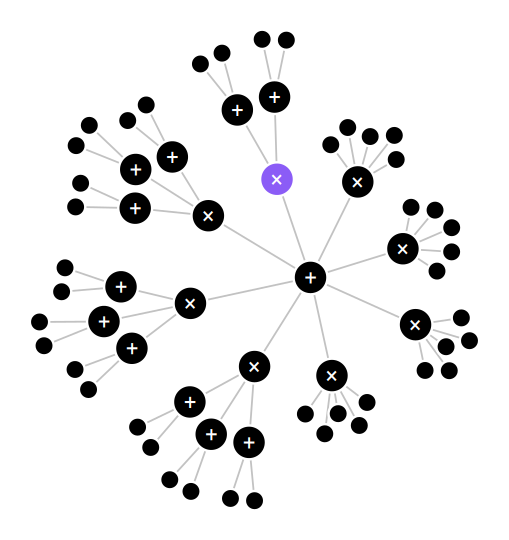
\includegraphics[width=0.5\textwidth]{images/K__5_5_-free__n_42_cotree.pdf}
    \caption{Cotree of a $K_{5,5}$-free extremal cograph on 42 vertices. The root is marked as purple. The corresponding cograph is the product of $K_{2,2}$ together with the sum of four $5$-cliques and three complete multipartite $K_{2,2,2}$.}
    \label{fig:cotree_example}
\end{figure}

The clique number behaves naturally with respect to cograph operations: $\omega(G_1 + G_2) = \max(\omega(G_1), \omega(G_2))$ and $\omega(G_1 \times G_2) = \omega(G_1) + \omega(G_2)$. Indeed, algebraically it can be seen as a valuation into the max-plus algebra.
This gives the bound
\begin{align}
    \text{height}(G) \leq 2 \cdot \omega(G) + 1. \label{eq:height_omega}
\end{align}

For $u \in V(T)$ let us denote the subtree of $u$ and its descendants with respect to the root of $T$ by $T(u)$. Let us transfer this notation to $G$ via
\begin{align}
    G(u) \coloneqq G[\mathscr{L}(u)],
\end{align}
where $\mathscr{L}(T(u))$ are the vertices that correspond to the leaves of $T(u)$.
It is easy to see that $G(u)$ is the cograph corresponding to the cotree $T(u)$.

\subsection{$(s,t)$-extremal cographs}

In this paper, we study the bipartite Tur\'an problem restricted to cographs.
For $s, t \in \NN$ with $s \leq t$, we call a cograph \emph{$(s,t)$-extremal} if it is edge-maximal among cographs not containing $K_{s,t}$.
By~\eqref{eq:height_omega}, any $(s,t)$-extremal cograph has height at most $2(s+t) - 1$.

In Figure \ref{fig:cotree_example} we present the typical symmetric structure of a $(5,5)$-extremal cograph on $42$ vertices, which we calculated using the algorithm introduced in Section \ref{subsec:dynamic_programming}.

\subsection{Our Contributions}\label{subsec:our_contributions}

We summarize our main contributions as follows.

\begin{itemize}[leftmargin=*, itemsep=0.35em]
    \item \textbf{Eventual linearity via pumping.}
    We prove a periodic \emph{Pumping Theorem} (Theorem~\ref{thm:pumping}) showing that for every fixed $s\le t$, extremal $K_{s,t}$-free cographs are obtained, for all sufficiently large $n$, by pumping a designated component inside one of finitely many core graphs; in particular,
\begin{align*}
    \mathrm{ex}\bigl(n,\{K_{s,t},P_4\text{-ind}\}\bigr)=a_{n\bmod R}+\alpha n
\end{align*}
    for all large $n$ and $\alpha = \frac{t-1}{2}$ in case $t \leq 2s - 1$.

    \item \textbf{A new lifting method for extremal cographs.}
    We introduce the \emph{lifting} procedure and formalize it in the Lifting Theorem (Lemma~\ref{thm:lifting}), which replaces suitable sums of components by a product of a small core with a sum of smaller graphs while preserving the biclique-profile constraint.
    This provides the key structural engine behind the pumping phenomenon and yields strong multiplicity restrictions on extremal decompositions.

    \item \textbf{Dynamic programming over cotrees and biclique-profiles.}
    Exploiting the recursive cotree structure of cographs, we develop a profile-based dynamic programming framework (Section~\ref{subsec:dynamic_programming}) to enumerate extremal cographs for small $n$ and to experimentally probe extremal structure (cf.\ Lemma~\ref{thm:profile_operations} and Definition~\ref{def:pareto_frontier}).

    \item \textbf{Complete classifications in special cases.}
    We give exact structural descriptions in several base regimes, including forbidden stars (Lemma~\ref{thm:pumping_stars}) and, most notably, a full characterization of $K_{3,3}$-free extremal cographs (Theorem~\ref{thm:classification_3_3}), enabling explicit enumeration of $(3,3)$-extremal cographs for every $n$.
\end{itemize}


\section{Biclique-Profiles}

For a graph $G$ let us define its \emph{biclique-sequence} by $\mathscr{S}(G)$, where for $s \in \NN$
\begin{align}
    \mathscr{S}_s(G) = \max \left\{ t \in \NN \ | \ K_{s,t} \subseteq G \right\}.
\end{align}
Here, we define $K_{0,t}$ as the empty graph on $t$ vertices, i.e., $\mathscr{S}_0(G) = |G|$. Observe that $\mathscr{S}_1(G)$ is the maximum degree.

Moreover, we define the maximum of the empty set as $-\infty$.
That is, the biclique-sequence of a graph is monotonically decreasing and constant $-\infty$ on indices greater than its vertex count. Furthermore, biclique-sequences are \emph{subdiagonal}, a property defined by the following two implications
\begin{alignat}{3}
    \mathscr{S}_{j}(G) < l 
    &\;\implies\;& K_{j, l} \nsubseteq G 
    &\;\implies\;& \mathscr{S}_{l}(G) < j \label{eq:subdiagonal_1},\\
    \mathscr{S}_{j}(G) \geq l 
    &\;\implies\;& K_{j, l} \subseteq G 
    &\;\implies\;& \mathscr{S}_{l}(G) \geq j \label{eq:subdiagonal_2}.
\end{alignat}
    
We might interpret $\mathscr{S}_{\infty}$ as the limit of the sequence, and deduce the following equivalence.
\begin{align}
    l = \mathscr{S}_{0}(G) < \infty &\iff \mathscr{S}_{l+1}(G) = -\infty \label{eq:finite_vertices_sequence}
\end{align}
Let us call any decreasing subdiagonal sequence $\mathscr{P}$ in $\NN \cup \{ \infty, -\infty \}$ a \emph{biclique-profile}.
Observe that a biclique-profile has $\mathscr{P}_0 < \infty$ if and only if it is constant $-\infty$ from some index onward.

Let us say a graph $G$ \emph{fulfills} a biclique-profile $\mathscr{P}$ in case that pointwise $\mathscr{S}(G) \leq \mathscr{P}$. Furthermore, a graph is \emph{extremal with respect to} $\mathscr{P}$ in case it fulfills $\mathscr{P}$ and it has the maximal edge count among all graphs with the same vertex count that fulfill $\mathscr{P}$.
We use the same notion for the extremal cograph problem.

The set of all biclique-profiles together with the element-wise ordering form a lattice with minimal element zero and the maximal element infinity.

For a biclique-profile $\mathscr{P}$ let us define its \emph{start index} by the minimal $i \in \NN_{0}$ such that $\mathscr{P}_i < \infty$. Similarly, we define its \emph{end index} as the minimal index where it attains its limit.
When considering extremal cographs not containing $K_{s,t}$ for $s \leq t$ observe that the corresponding biclique-profile has start index $s$, where it attains the value $t-1$, and stop index $t$ where it jumps to its limit $s-1$.
In the following Lemma we make use of the so-called "lifting" procedure, where we replace the sum of components in an extremal structure by a product of a small core and the sum of smaller structures.

\begin{Lemma}[Lifting Theorem] \label{thm:lifting}
    Let $\mathscr{P}$ be a biclique-profile with start index $s$ such that $\mathscr{P}_s = t-1$. Let $n \in \NN$. For any cograph $G$ on $n$ vertices that is extremal with respect to $\mathscr{P}$ there is a finite index set $I$ and a mapping $\sigma: I \to [t-1]$ such that:
    \begin{enumerate}[label=(\roman*)]
        \item $G$ admits the decomposition:
        \begin{align}
            G = \sum_{i \in I} G_{i,1} \times G_{i,2} \label{eq:lifting_mapping}
        \end{align}
        where $|G_{i,1}| = \sigma(i)$ and $|G_{i,2}| \geq \sigma(i)$ for all $i \in I$.
        \item For any $1 \leq j \leq s-1$, the fiber $|\sigma^{-1}(j)| \leq 1$.
        \item In case $t \leq 2s - 1$ there exists a constant $c(s,t)$ such that for any $1 \leq j \leq t-1$ the fiber $|\sigma^{-1}(j)| \leq c(s,t)$.
    \end{enumerate}

    We remark that in case $2 \leq s  \leq t \leq 2s - 1$ (ii) and (iii) together imply that there are only finitely many connectivity components in $G$.
\end{Lemma}

\begin{proofref}{Lemma}{thm:lifting}   
    Let $G$ be a cograph on $n$ vertices extremal with respect to $\mathscr{P}$.
    Since $G$ is a cograph, each connectivity component $C_i$ for $i \in I$ is a product. We write $C_i = G_{i,1} \times G_{i,2}$ and choose the decomposition such that $\sigma(i) \coloneqq |G_{i,1}|$ is minimal. Note that $\sigma(i) < t$ must hold. If not, $|G_{i,1}| \geq t$ and $|G_{i,2}| \geq t$, implying $K_{t,t} \subseteq C_i$. As $s \leq t$, this implies $K_{s,t} \subseteq G$, which violates the start index condition $\mathscr{P}_s = t-1$.
    
    To prove (ii), assume for a contradiction that there exist distinct indices $i_1, i_2 \in I$ such that $\sigma(i_1) = \sigma(i_2) = j$ for some $j \in [s-1]$. Now we continue by a lifting argument.
    
    Consider the cograph $G'$ formed by replacing the components $C_{i_1} + C_{i_2}$ with a single component:
    \begin{align*}
        C' \coloneqq E_j \times (G_{i_1,2} + G_{i_2,2} + K_j).
    \end{align*}
    This graph $G'$ has the same vertex count as $G$. We claim $G'$ still fulfills $\mathscr{P}$.

    Let $s' \geq s$ and $p \coloneqq \mathscr{P}_{s'}$.
    It is clear that $p \geq s-1$ as otherwise by (\ref{eq:subdiagonal_1}) $\mathscr{P}_{s-1} < \infty$, a contradiction to the definition of $s$ as the start index. Hence any biclique that would violate $\mathscr{P}$ has size at least $2s$.
    
    It is clear that $G'$ does not contain $K_{s', p+1}$ unless the product $C'$ does contain it. However, this could only be the case if $E_j \times K_j$ does contain it, which is not possible as $2s = 2s > 2 j$.
    
    Furthermore, $G'$ has strictly more edges than the sum $C_{i_1} + C_{i_2}$.
    Indeed, the cross edges between $G_{i_2, 1}$ and $G_{i_2, 2}$ are covered by the edges between $E_j$ and $G_{i_2, 2}$.
    Moreover, $\| G_{i_1, 1} \| \leq K_j$ and the remaining cross edges exceed the edges inside $\| G_{i_2, 1} \|$ as $j^2 < \binom{j}{2}$ - $\| G_{i_2, 1} \| < \| E_j, K_j \|$.
    This contradicts the edge-maximality of $G$.

    To prove (iii) we use a similar lifting argument. Let us assume that $t \leq 2s - 1$ and fix $s \leq j \leq t-1$.
    % As there are only finitely many cographs on $j$ vertices, we may assume that there is a cograph $G_1$ such that all $i \in \sigma^{-1}(j)$ have the same smaller multiplicative component $G_{i,1} = G_1$. By its minimality we know that $G_1$ is not complete.

    We may similarly construct $G'$ by replacing $C \coloneq \sum_{i \in \sigma^{-1}(j)} C_i$ by
    \begin{align}
        C' \coloneqq E_{s-1} \times \left( \sum_{i \in \sigma^{-1}(j)} G_{i,2} + (|\sigma^{-1}(j)| - 1) \cdot K_j + K_{j-s+1} \right).
    \end{align}

    In order to see that $C'$ fulfills $\mathscr{P}$ it suffices to show this for $E_{s-1} \times K_j$ and $E_{s-1} \times K_{j-s+1}$.
    
    Again the fact that any biclique contradicting $\mathscr{P}$ would need to have at least $2s$ trivially yields that $E_{s-1} \times K_{j-s+1}$ fulfills $\mathscr{P}$ as $j < t \leq 2s - 1 < 2s$.
    Moreover, in $E_{s-1} \times K_j$ the largest bicliques are $K_{s-1, j}$ and $K_{q, j-q}$ for $1 \leq q \leq j-1$. Hence, also $E_{s-1} \times K_j$ fulfills $\mathscr{P}$.

    We may show that $C'$ contains more edges than $C$.
    It is clear that by the minimality of $G_{i,1}$ none of the $G_{i,1}$ are complete.
    Thus, in case $|\sigma^{-1}(j)| - 1 > \binom{s-1}{2}$, the edges in the $j$-cliques on the right make up for missing edges in $E_{s-1}$ compared to $G_{i,1}[X_{i}]$.

    By the same argument it is left to show that there the difference of the counts of cross edges in $C'$ and $C$ is at most constant.
    Compared to $C$ by making the left part of the product smaller we lost $(j-s+1)|G_{i,2}|\leq (j-s+1)(t-1)$ edges for each $i \in \sigma^{-1}(j)$.
    However, we gained $(s-1)\left( (j-s+1) + (|\sigma^{-1}(j)| - 1) j \right)$ edges.

    Thus, the count of lost cross edges in the lifting stays constant if $(s-1)j \geq (j-s+1)(t-1)$, which simplifies to
    \begin{align}
        j \leq \frac{(s-1)(t-1)}{t-s}.
    \end{align}
    
    We remark that this condition is true for all relevant $j \leq t-1$ if and only if $s-1 \geq t-s$, i.e. $t \leq 2s-1$.
\end{proofref}

\subsection{Dynamic programming} \label{subsec:dynamic_programming}

The recursive structure of cographs via sum and product operations naturally leads to a dynamic programming approach for computing extremal graphs.
We first observe that biclique-sequences combine predictably under these operations.

\begin{Lemma}[Profile operations] \label{thm:profile_operations}
    Let $G_1, G_2$ be cographs on $n_1, n_2$ vertices respectively. Then:
    \begin{enumerate}[label=(\roman*)]
        \item For the sum $G_1 + G_2$:
        \begin{align}
            \mathscr{S}_s(G_1 + G_2) = \max\left(\mathscr{S}_s(G_1), \mathscr{S}_s(G_2)\right) \label{eq:profile_sum}
        \end{align}
        \item For the product $G_1 \times G_2$:
        \begin{align}
            \mathscr{S}_s(G_1 \times G_2) = \max_{a+c=s}\left(\mathscr{S}_a(G_1) + \mathscr{S}_c(G_2)\right) \label{eq:profile_product}
        \end{align}
    \end{enumerate}
\end{Lemma}

\begin{proofref}{Lemma}{thm:profile_operations}
    (i) In a sum $G_1 + G_2$, there are no edges between $V(G_1)$ and $V(G_2)$. Thus any $K_{s,t} \subseteq G_1 + G_2$ must lie entirely in $G_1$ or entirely in $G_2$, giving the pointwise maximum.

    (ii) In a product $G_1 \times G_2$, every vertex in $G_1$ is adjacent to every vertex in $G_2$. A copy of $K_{s,t}$ can use $a$ vertices from one side of the biclique in $G_1$ and $c = s - a$ vertices from the other side, with the remaining vertices coming from $G_2$. The maximum over all such decompositions yields the max-convolution formula.
\end{proofref}

The key observation is that the number of edges also combines predictably:
\begin{align}
    \|G_1 + G_2\| &= \|G_1\| + \|G_2\| \label{eq:edges_sum} \\
    \|G_1 \times G_2\| &= \|G_1\| + \|G_2\| + n_1 \cdot n_2 \label{eq:edges_product}
\end{align}

We say a biclique-profile $\mathscr{P}$ \emph{dominates} another profile $\mathscr{P}'$ if $\mathscr{P}_i \geq \mathscr{P}'_i$ for all $i \in \NN_0$, and write $\mathscr{P} \geq \mathscr{P}'$.
This defines a partial order on profiles, which forms a lattice structure.

\begin{Definition}[Pareto frontier] \label{def:pareto_frontier}
    For a set of pairs $\{(\mathscr{P}_j, e_j)\}_{j \in J}$ consisting of biclique-profiles and edge counts, the \emph{Pareto frontier} is the set of pairs $(\mathscr{P}_j, e_j)$ such that there is no other pair $(\mathscr{P}_k, e_k)$ with $\mathscr{P}_k \leq \mathscr{P}_j$ (coordinatewise) and $e_k \geq e_j$, with at least one strict inequality.
\end{Definition}

For computing extremal cographs, we observe that dominated profile-edge pairs can never contribute to an extremal graph: if $(\mathscr{P}, e)$ is dominated by $(\mathscr{P}', e')$ with $\mathscr{P}' \leq \mathscr{P}$ and $e' \geq e$, then any graph fulfilling $\mathscr{P}$ also fulfills $\mathscr{P}'$, and the dominating graph has at least as many edges.

The algorithm proceeds by dynamic programming over the vertex count $n$. For each $n$, we maintain a registry $\mathcal{R}_n$ of pairs $(\mathscr{P}, \mathcal{G}_{\mathscr{P}})$, where $\mathcal{G}_{\mathscr{P}}$ is the set of cographs on $n$ vertices having profile $\mathscr{P}$ with maximum edge count among graphs with that profile.

\begin{center}
\fbox{\parbox{0.9\textwidth}{
\textbf{Algorithm: Dynamic Programming for Extremal Cographs}
\begin{enumerate}[label=\arabic*.]
    \item \textbf{Base case.} Set $\mathcal{R}_1 \leftarrow \{((1, 0, \ldots), \{K_1\})\}$.

    \item \textbf{Inductive step.} For each $n \geq 2$:
    \begin{enumerate}[label=(\alph*)]
        \item Initialize candidate set $\mathcal{C}_n \leftarrow \emptyset$.
        \item For each partition $n = n_1 + n_2$ with $1 \leq n_1 \leq n_2$:
        \begin{enumerate}[label=(\roman*)]
            \item For each $(\mathscr{P}_1, \mathcal{G}_1) \in \mathcal{R}_{n_1}$ and $(\mathscr{P}_2, \mathcal{G}_2) \in \mathcal{R}_{n_2}$:
            \begin{itemize}
                \item Compute $\mathscr{P}_{+} = \mathscr{S}(\mathscr{P}_1 + \mathscr{P}_2)$ via~\eqref{eq:profile_sum}.
                \item Compute $\mathscr{P}_{\times} = \mathscr{S}(\mathscr{P}_1 \times \mathscr{P}_2)$ via~\eqref{eq:profile_product}.
                \item Compute edge counts $e_{+}$, $e_{\times}$ via~\eqref{eq:edges_sum}--\eqref{eq:edges_product}.
                \item Add $(\mathscr{P}_{+}, e_{+}, G_1 + G_2)$ and $(\mathscr{P}_{\times}, e_{\times}, G_1 \times G_2)$ to $\mathcal{C}_n$ for each $G_1 \in \mathcal{G}_1$, $G_2 \in \mathcal{G}_2$.
            \end{itemize}
        \end{enumerate}
        \item \textbf{Pareto filtering.} Reduce $\mathcal{C}_n$ to the Pareto frontier with respect to the partial order $(\mathscr{P}, e) \preceq (\mathscr{P}', e')$ iff $\mathscr{P} \geq \mathscr{P}'$ and $e \leq e'$.
        \item Group by profile: $\mathcal{R}_n \leftarrow \{(\mathscr{P}, \{G : (\mathscr{P}, e, G) \in \mathcal{C}_n, e = e_{\max}(\mathscr{P})\})\}$.
    \end{enumerate}

    \item \textbf{Query.} Given a biclique-profile $\mathscr{P}$ with $\mathscr{P}_0 = n$, return graphs from $\mathcal{R}_n$ whose profiles are $\leq \mathscr{P}$ (coordinatewise) with maximum edge count.
\end{enumerate}
}}
\end{center}

The lattice-based optimization (step 2c) prunes dominated profile pairs at the profile level \emph{before} expanding to individual graph pairs, reducing the combinatorial explosion.
For a partition $(n_1, n_2)$ with $|\mathcal{R}_{n_1}| = p_1$ and $|\mathcal{R}_{n_2}| = p_2$ profiles, the naive approach considers $O(p_1 \cdot p_2 \cdot g_1 \cdot g_2)$ graph pairs, where $g_1, g_2$ are the average number of graphs per profile.
The lattice filtering first computes the antichain of non-dominated profile pairs (at most $O(p_1 \cdot p_2)$), then only expands graph pairs for surviving profile combinations.

For practical computation with a pruning constraint $K_{s,t}$, we can truncate profiles to length $s+1$ since only the first $s$ entries determine whether a graph fulfills the constraint $\mathscr{P}_s < t$. Moreover, when only interested in $(a,b)$-extremal graphs we can prune all profiles $\mathscr{P}$ where $\mathscr{P}_a \geq b$.

It is easy to see that our approach is correct: In an $(s,t)$ extremal graph all components are extremal with respect to a biclique profile that depends on the remaining graph. Thus, by combining all graphs extremal to suitable profiles, the search considers all relevant candidates for extremal cographs.

By step (c) we lose the ability to enumerate all extremal graphs. We remark that one could simply skip step (c) - at the cost of significantly more memory consumption and run time. However, it is easy to see that also with step (c) one still finds at least one extremal graph for each $n \in \NN$.

\section{Main Results}

\subsection{Special cases}

Before we consider the general case, it is instructive to consider two special and simpler cases, where it is easy to enumerate all extremal graphs for all $n \in \NN$.
We already use ideas that however work out simpler with small parameters than in the general case.

\begin{Theorem} \label{thm:classification_2_t}
    Let $t \in \NN$ with $t \geq 2$ and let $G$ be a $(2,t)$-extremal cograph on $n \geq 2$ vertices that does not contain $K_{2,t}$.
    Then, $G$ is the product of a vertex with another cograph $G_2$ of maximal degree $t-1$.
\end{Theorem}

\begin{proofref}{Theorem}{thm:classification_2_t}
    Let $G$ be a $(2,t)$-extremal cograph on $n$ vertices. Let $H_1, \dots, H_l$ be its connectivity components. Any of it is a product of a vertex $v_j$ with some cograph $H_j'$ (which might be empty in case of singletons).

    However, the Lifting Theorem \ref{thm:lifting} yields that there only could be one such component, yielding that $G$ is connected and $G = v \times G'$. It is evident that the maximal degree in $G'$ is at most $t-1$.
\end{proofref}

\begin{Theorem}\label{thm:classification_3_3}
    Let $G$ be an edge-maximal cograph on $n \geq 2$ vertices that does not contain $K_{3,3}$. Then, $G$ is the product of a two-vertex cograph $G_1$ with another cograph $G_2$. Moreover, there is always an edge-maximal cograph on $n \geq 2$ vertices such that $G_1$ is an edge and $G_2$ is the sum of cliques.  
\end{Theorem}

\begin{proofref}{Theorem}{thm:classification_3_3}
    Let us prove the claim by induction on $n$.
    In case that $2 \leq n < 6$ it is clear that $G$ is a clique and therefore the product of an edge with another cograph. This solves the base case.
    
    \textbf{step.} We might assume that $n \geq 6$.
        First, let us prove that $G$ is connected. Assume for a contradiction that $G = H_1 + H_2$ for two cographs $H_1$ and $H_2$.
        Then, either $H_1 \geq 2$ and induction yields that we might replace $H_1$ by an edge-maximal cograph not containing $K_{3,3}$ that has a complete vertex $v_1$. Otherwise, $H_1$ itself is a singleton and a complete vertex itself. The same argument yields a complete vertex $v_2$ of $H_2$. However,
        \begin{align}
            \tilde{G} \coloneqq v_1 \times \left( \left( H_1 - v_1 \right) + \left( H_2 - v_2 \right) + v_2 \right)
        \end{align}
        has one more edge than $G$ and also does not contain $K_{3,3}$, a contradiction.

        Hence, we know that $G = H_1 \times H_2$ for two cographs $H_1$ and $H_2$ on $n_1$ and $n_2$ vertices respectively.
        Let us assume that $n_1 \leq n_2$. Moreover, we might assume that our choices of $H_1$ and $H_2$ maximize $n_1$ under this restriction.
        It is clear that $n_1 < 3$, so to show $n_1 = 2$ we only need to show that $n_1 \neq 1$.
        
        Let us assume for a contradiction that $H_1$ is made of a single vertex $v$. Since we assumed $H_1$ to be maximal under the restriction $n_1 \leq n_2$, we might assume that $H_2 = \sum_{j \in [l]} H_{2,j}$. However, it is easy to see that each $H_{2,j}$ is $(2,3)$-extremal so Theorem \ref{thm:classification_2_t}
        yields a complete vertex $v_{j}$ in $H_{2,j}$.
        However,
        \begin{align}
            \tilde{G} \coloneqq v \times v_1 \times \left( \sum_{j \in [l]} \left( H_j - v_j \right) + \sum_{j \in [l]\setminus\{1\}} v_j \right)
        \end{align}
        does not contain $K_{3,3}$ and has $l-1$ more edges than $G$, a contradiction.

        Thus, we know that $H_1$ does contain two vertices. It is left to show that there is an extremal graph $G$ with two complete vertices, i.e. the respective $H_1$ is an edge.

        It is clear that $H_2$ does not contain a $K_{1,3}$.
        \begin{Claim} \label{claim:13}
            Any edge-maximal cograph $G$ not containing $K_{1,3}$ is the sum of cliques of size at most $3$ and four-cycles.
        \end{Claim}

        \begin{proofref}{Claim}{claim:13}
            It is easy to see that any connectivity component of $G$ can have at most $4$ vertices. It is easy to check manually that indeed, for any vertex count of at most $4$ any edge-maximal and connected cograph not containing $K_{1,3}$ is either a clique or a four-cycle.
            This concludes the proof of Claim \ref{claim:13}.
        \end{proofref}

        Claim \ref{claim:13} yields that $H_2$ is the sum of cliques of size at most $3$ and four-cycles.
        We might assume that it is the sum of $a$ triangles, $b$ four-cycles, and a clique of size $s \in \{ 0, 1, 2 \}$.
        Then,
        \begin{align}
            \| H_2 \| = 3 \cdot a + 4 \cdot b + \mathbb{1}\{ s = 2 \}
        \end{align}
        In case that $H_2$ does not contain a four-cycle, by edge-maximality it is clear that $H_1$ is an edge.
        In case that $H_2$ does contain a four-cycle, $H_1$ cannot be an edge, as otherwise a $K_{3,3}$ would arise.
        Let us check all cases to see that in case $H_2$ does contain a four-cycle, we can replace the four-cycles with cliques and $H_1$ by an edge and obtain a $K_{3,3}$-free graph of the same edge count. We might replace $H_2$ by any edge-maximal sum of triangles, four-cycles, edges, and singletons for the given vertex count.

        \textbf{case $n_2 \ \text{mod} \ 3 = 0$.} In this case, $H_2$ can be chosen to be made out of triangles and $H_1$ would be an edge.

        \textbf{case $n_2 \ \text{mod} \ 3 = 1$.} In this case $H_2$ can be chosen to be made of triangles and either a singleton (in case $n_2 = 4$) or a single four-cycle. In the first case, $H_1$ is an edge. In the latter case we can replace the four-cycle by a triangle and a singleton and add the edge in $H_1$ for compensation.

        \textbf{case $n_2 \ \text{mod} \ 3 = 2$.}  In this case $H_2$ can be chosen to be made of triangles and either an edge (in case $n_2 = 5$) or two four-cycles. In the first case, $H_1$ is an edge. In the latter case, we can replace the two four-cycles by two triangles and an edge and add the edge in $H_1$ for compensation.

        This completes the proof of Theorem \ref{thm:classification_3_3}.
\end{proofref}

In the sequel we are going to use the so-called \emph{Davenport Theorem}.

\begin{Theorem}[Davenport] \label{thm:davenport}
    For any $n \in \NN$, let $A$ be a sequence of $n$ integers. There exists a non-empty subsequence of $A$ whose sum is divisible by $n$.
\end{Theorem}

\begin{Lemma}[Forbidden stars] \label{thm:pumping_stars}
    Let $t,n \in \NN$. There is $C$ such that any $(1,t)$-extremal cograph on $n$ vertices is the sum of $(t-1)$-regular cographs and remainder of size at most $C$. In case $t$ is odd, for $n \geq (t-1)(2t-3)$ all $(1,t)$-extremal graphs are sums of $(t-1)$-regular cographs.
\end{Lemma}

\begin{proofref}{Lemma}{thm:pumping_stars}
    Let us choose $C \coloneqq 2(t-1)^2$.
    Let $n \in \NN$ and $G$ be a $(1,t)$-extremal graph. That is, it has maximum degree at most $t-1$.

    Let $C_1, \dots, C_l$ be its connectivity components. For any $i \in [l]$ there are $G_{i,1}$ and $G_{i,2}$ such that $C_i = G_{i,1} \times G_{i,2}$. As $|G_{i,1}| \leq t-1$ and $|G_{i,2}| \leq t-1$ it is apparent that $|C_i| \leq 2(t-1)$.

    As there are finitely many cographs $\Omega$ on at most $2(t-1)$ vertices and maximum degree at most $t-1$, the graph $G$ maximizes the edge count in an unbounded knapsack-like problem, where the items are $\Omega$, the cost function is their vertex count, and the value function is their edge count.

    Let us assume for a contradiction that there is $l' \geq 2$ such that $C_1,\dots,C_{l'}$ are the non-regular components and their total size exceeds $C$. It is clear that $l' \geq t$. Thus, the Davenport Theorem \ref{thm:davenport} yields non-empty $X \subseteq [l']$ such that $t$ divides $\sum_{j \in X} |C_j|$. Thus, we can replace $\sum_{j \in X} C_j$ by $t$-cliques. As $t$-cliques are $t$-regular, the resulting graph has more edges, a contradiction.

    In case $t$ is odd, observe that both $K_t$ and $K_{t-1, t-1}$ are $(t-1)$-regular and as the greatest common divisor of their vertex count is one,
    \begin{align}
        \text{gcd}\left( t, 2(t-1) \right) = 1,
    \end{align}
    it follows by a result of Sylvester \citep{Sylvester1882} about the Frobenius coin problem that for any $n \geq (t-1)(2t - 3)$ there are $a,b \in \NN$ such that $n = at + 2b(t-1)$. Thus, $a\cdot K_t + b \cdot K_{t-1, t-1}$ is an $(1,t)$-extremal cograph and it is evident that any such extremal cograph can only have $(t-1)$-regular connectivity components.
\end{proofref}

We want to remark that for example all complete multipartite graphs with equally sized partition classes are connected regular cographs. However, there are many more, as there are even connected regular cographs with different vertex degrees in different multiplication components---consider the $4$-regular cograph $2K_2 \times E_3$. Interestingly, Allem, Chen, and Tura~\cite{Allem2023} recently proved that regular cographs are determined by their Laplacian spectrum, highlighting the rigid spectral structure of this family.

\subsection{The general Pumping Theorem}

\begin{Theorem}[Pumping Theorem] \label{thm:pumping}
    Let $s, \ t \in \NN$ with $s \leq t$.
    There is $\alpha > 0$ and $R, N \in \NN$ and core graphs $G_j$ with components $H_j \subseteq G_j$ of edge density $\alpha$ such that for any $n \geq N$ there is an extremal graph on $n$ vertices that is constructed by pumping $H_{(n \ \text{mod} \ R)}$ inside of $G_{(n \ \text{mod} \ R)}$.
    That is, for $n \geq N$
    \begin{align}
        \text{ex}(n, \{K_{s,t}, P_4\text{-ind}\}) = a_{(n \ \text{mod})} + \alpha n.
    \end{align}

    Moreover, in case that $t \leq 2 s-1$, the pumping component $H_j$ has a common neighbourhood in $G_j$ of size $s-1$ and the pumping components are $(t-1)$-regular, i.e. $\alpha = \frac{t-1}{2}$.
\end{Theorem}

\begin{proofref}{Theorem}{thm:pumping}
    In case $s=1$, the statement follows from Lemma \ref{thm:pumping_stars}. Hence, let us assume that $s \geq 2$.
    Let us fix $D \coloneqq 4t^2 + s$ and $N \coloneqq D ^ {2(s+t) + 1} + 1$.
    Let $G$ be an $(s,t)$-extremal cograph on $n \geq N$ vertices. Let $T_G$ be its reduced cotree.
    
    \textbf{1. Bounded degree of product vertices:}
    Let $u$ be any product vertex in $T_G$. Let $v_1, \dots, v_k$ be its children. Since $G$ is a cograph, the subgraph induced by $u$ contains a complete multipartite graph with parts of sizes $|G(v_1)|, \dots, |G(v_k)|$. Since every child in the cotree has at least one vertex, if $k \geq s+t$, one could find a $K_{s,t}$ in $G$. Thus, any product vertex has strictly less than $s+t \leq D$ children.
    
    \textbf{2. Existence of a high degree addition vertex:}
    Let us assume for a contradiction that all addition vertices have at most $D$ children. By (\ref{eq:height_omega}) it is clear that $\text{height}(G) \leq 2(s+t) + 1$. This implies however that $n \leq D ^ {2(s+t) + 1}$, a contradiction.
    Thus, we know that there exists a vertex $v$ with at least $D+1$ children.
    
    \textbf{3. Structure of $G(u)$ for addition vertices $u$:}
    Let $u$ be an addition node.
    All vertices in $G(u)$ have the same neighborhood $W$ in $G \setminus G(u)$. Since $|G(u)| \geq t$ it is clear that $w \coloneqq |W| < s$.
        
    Observe that $G(u)$ is extremal with respect to some biclique-profile $\mathscr{P}^{(u)}$ with start index $s-w$.
    
    By Lemma \ref{thm:lifting} (ii) any addition vertex has at most $s-w-1$ children $X^{(u)}_1$ such that for $x \in X^{(u)}_1$ there could be a large $G(x)$. All other children $X^{(u)}_2$ have size at most $2 \cdot \mathscr{P}^{(u)}_{s-w} < 2t$.

    \textbf{4. Reduction to a core graph with one pumped component:}
    Let us assume that $v$ has $d > D$ children. Then, $|X^{v}_2| > d - |X^{v}_2| > D - s = 4t^2$.
    As for $x \in X^{v}_2$ by definition $|G(x)| < 2t$ by the pigeonhole principle there is one $q \in [2t]$ such that there are at least $2t$ vertices $X_{\text{pump}} \subseteq X^{(v)}_2$ such that for any $x \in X'$ we have $|G(x)| = q$.
    
    Let us denote the addition vertices with more than $D$ children by $V^+$ and let us denote all the children of such addition vertices that correspond to small components except $X_{\text{pump}}$ by
    \begin{align}
        X_{\text{pool}} \coloneqq \bigcup_{u \in V^+} X^{(u)}_2 \setminus X_{\text{pump}}.
    \end{align}

    Now for any $x \in X_{\text{pool}}$ we may choose an arbitrary subset $X_{\text{test}} \subseteq X_{\text{pump}}$ of size $\mathscr{L}(x)$ and replace the vertices $\bigcup_{y \in X_{\text{test}}} \mathscr{L}(y)$ by $q$ times duplicating $G(x)$ to obtain a graph $G'$ of the same vertex count.
    As all vertices in $V^+$ have more than $t$ descendant leaves, we know that their pairwise common descendants are addition vertices. Hence, also $G'$ does not contain a $K_{s,t}$.
    This implies that
    \begin{align}
        \| G' \| \leq \| G \|. \label{eq:move_inequality}
    \end{align}

    For $z \in V(T)$ let us introduce the notation
    \begin{align}
        e(z) \coloneqq \left\| G(z) \right\| + \left\| \mathscr{L}(z), V(G) \setminus \mathscr{L}(z) \right\|.
    \end{align}
    It is clear that for any $x_1, x_2 \in X_{\text{pump}}$ we have $e(x_1) = e(x_2)$, let us denote it by $e_{\text{pump}}$.
    Moreover, we may replace all $G(x_2)$ by one of the components, let us denote it by $G_{\text{pump}}$.
    Moreover, by (\ref{eq:move_inequality}) we have
    \begin{align}
        q \cdot e(x) \leq |\mathscr{L}(x)| \cdot e_{\text{pump}}.
    \end{align}

    Now, for any $X_{\text{candidates}} \subseteq X_{\text{pool}}$ of size $q$ by Davenport's Theorem \ref{thm:davenport} we find $X_{\text{replace}} \subseteq X_{\text{candidates}}$ such that $q$ divides $\sum_{x \in X_{\text{replace}}} e(x)$, let us say by $r$.
    As
    \begin{align}
        q \cdot \sum_{x \in X_{\text{replace}}} e(x)
            \leq e_{\text{pump}} \cdot \sum_{x \in X_{\text{replace}}} |\mathscr{L}(x)|
    \end{align}
    we conclude that
    \begin{align}
        \sum_{x \in X_{\text{replace}}} e(x) \leq e_{\text{pump}} \cdot r.
    \end{align}
    This shows that we may replace $\bigcup_{x \in X_{\text{replace}}} \mathscr{L}(x)$ by $r$ copies of $G_{\text{pump}}$ without losing edges.
    However as $D \geq t$ this also gives no rise to a $K_{s,t}$.

    Iterating this procedure, we arrive at an $(s,t)$-extremal cograph $G'$, where all vertices except $v$ have at most $D$ children, except for at most $q-1$ leftover children from $X_{\text{pool}}$.
    For ease of notation let us assume that $G=G'$.
    
    Now, let us consider the graph $G_{\text{core}}$ obtained by deleting $\bigcup_{x \in X_{\text{pump}}} \mathscr{L}(x)$.
    It has at most $N_{s,t} \coloneqq D^{2(t+s)+1} + q \cdot 2t$ vertices.
    Moreover, it is $(s,t)$-free.

    \textbf{5. Cyclic repetition of the core graphs:}
    For any cograph of size at most $N_{s,t}$ there is a finite number of children $x$ of addition vertices, so that one can blow up $G(x)$ indefinitely so that the resulting cograph does not contain $K_{s,t}$.
    This gives a finite number of equation restriction pairs of the form
    \begin{align}
        a_j + b_j \cdot n, \ n \ \text{mod} \ q_j = \gamma_j,
    \end{align}
    for $j \in \Omega$ that correspond to a cograph $G_j$ on at most $N_{s,t}$ vertices together with the child of an addition vertex $u_j \in V(G_j)$ that would be pumped. Observe that $q_j = |\mathscr{L}(u_j)|$ and $\gamma_j = |G_j| \text{mod} q_j$
    Then, for $n \geq N_{s,t}$
    \begin{align}
        \text{ex}\left( n, \left\{ K_{s,t}, P_4 - \text{ind} \right\} \right) = \text{max} \left\{ a_j + b_j \cdot n \ | \ j \in \Omega, \ n \ \text{mod} \ q_j = \gamma_j \right\}.
    \end{align}

    As for large $n$ the linear part $b_j \cdot n$ takes over the constant $a_j$ there is $N, R$ and $\sigma: \ \ZZ \textfractionsolidus R\ZZ \longrightarrow \Omega$ such that for any $n \geq N$
    \begin{align}
        \text{ex}\left( n, \left\{ K_{s,t}, P_4 - \text{ind} \right\} \right) = a_{\sigma(n \ \text{mod} R)} + b_{\sigma(n \ \text{mod} R)} \cdot n.
    \end{align}

    Moreover, we know that there is $\beta$ such that for any $j \in \ZZ \textfractionsolidus R \ZZ$ we have $b_j = \beta$. Otherwise, there are distinct $j_1, j_2 \in \ZZ \textfractionsolidus R \ZZ$ such that $\frac{b_{j_1}}{q_{j_1}} < \frac{b_{j_2}}{q_{j_2}}$. Thus we could 'shift' the pumped up $G_{\sigma(j_2)}$ into the right vertex count modulo class $j_1$ with respect to $R$ by adding singletons. For large $n$ this leads to a contradiction, as the linear term of the extremal number surpasses the constant term.

    \textbf{5. The pumping structure in case $t \leq 2s - 1$:}
    Let us assume for now that $t \leq 2s - 1$.
    Fix $j \in \ZZ \textfractionsolidus R\ZZ$. We want to analyze the structure of the pumping component $G_{\sigma(j)}$.

    Let $W \coloneqq \mathscr{N}\left( \mathscr{L}(u_{\sigma(j)}) \right)$ be the common neighbourhood of the pumping component in the core graph.
    Let us assume for a contradiction that $w \coloneq |W| \leq s-2$.

    There exists a biclique-profile $\mathscr{P}^{(j)}$ such that $G(u_{\sigma(j)})$ is extremal with respect to $\mathscr{P}^{(j)}$. This biclique-profile has start index $s-w$ and $\mathscr{P}^{(j)}_s = t-w-1$.

    Now, as $t-w \leq 2s - 1 - w \leq 2(s-w) - 1$ we may apply the Lifting Theorem \ref{thm:lifting} with starting index $s-w$ and start value $t-w-1$, where the condition for (iii) is fulfilled. As we assumed that $s-w \geq 2$, it yields that any extremal cograph with respect to $\mathscr{P}$ has only finitely many connectivity components, a contradiction in case of large $n$.    
\end{proofref}

\section{Conclusion}

We have shown that the bipartite Turán problem on cographs admits an exact linear solution for large $n$, characterized by a periodic "pumping" of specific dense components. This contrasts with the general bipartite Turán problem, where bounds are polynomial but not linear. The strong structural constraints of cographs (bounded clique-width, bounded VC-dimension) force the extremal graphs into a rigid algebraic shape.

An interesting open question is whether the restriction $t \le 2s-1$ used in the Lifting Theorem is necessary for the finite component decomposition, or if it is an artifact of the proof method. We conjecture that the periodicity sets in much earlier than our bounds suggest, as we found no small counterexamples in extensive searches of small extremal cographs with $s,t \leq 12$ and $n \leq 80$.

Finally, we want to remark that the exact determination of $\text{ex}\left( n, \left\{ H, P_4 - \text{ind} \right\} \right)$ is still an unsolved and interesting problem for $H$ that is neither a clique nor a biclique.

\bibliographystyle{plainnat}
\bibliography{references}

\end{document}